\chapter{Test Results}

To understand how well the trained agent performs, training results are not enough since they only provide information about how well rewarded the agent is, and not about how it will perform in a real environment. For this, several tests were set up for the 3 types of problems that were tackled in this paper.


\section{Reaching a static target}

For reaching a static target, the test consists of an agent that has to touch 40 targets that are static (i. e. not moving) and that appear in a predefined order. Once the agent touches the target, it disappears and a new one appears in a new location, according to the predefined order. For each test, the same predefined order of targets is used so that the test course is the same for each run. 

Initially, this test was done using only agents that were trained to reach static targets, however a more robust experiment would be to also run the test using agents that were trained to reach moving targets, and compare the results at the end.


\subsection{Agent trained to reach static targets}

The results for testing the agent that was trained to reach static targets can be seen in Table \ref{move_to_static_target_test_results:1} and Figure \ref{test_results_static_target_static_brain_bar_chart}. It can be observed that, unlike the training results, using a smaller network architecture does not yield better times, with the architecture with 5 hidden layers and 128 units per layer being the one that achieved the best time, 170.9822 s. For the architecure with a single hidden layer, the configuration with 128 units was faster by 22.66 s ($11.01\%$) than the one with 512 units per layer. Since the configuration with 256 units per layer was unable to be trained, because it learned just to move in a circle, it was unable to finish the test course.

For the architecture with 3 hidden layer, the results were much more similar, with the configurations that had 256 and 512 units per layer, having virtually identical times, with the difference between them being 0.2 seconds, and the configuration with 128 units being slower than these two by 2 seconds ($\sim1\%$ slower). These results are somewhat surprising since there was a differnce of $29\%$ in the training performance of the configuration with 128 units compared to the one with 512 units.

The architecture with 5 hidden layers has the configuration that is the best performing in this test, the one with 128 units per layer, which manages to achieve a time of 170.9822 seconds. The other two configurations perform worse, the one with 256 units being slower by 15.4805 seconds ($\sim8.3\%$ slower), and the one with 512 units being slower by 34.8443 seconds ($\sim16.92\%$ slower). This shows that a smaller number of layers does not necessarily lead to better results, however, using less units per hidden layer usually means that the agent will perform better.

The final network architecture, the one with 7 layers has the configuration with 256 units be the fastest one in the test, clocking in at 182.1618 seconds. The configuration with 128 units was slower by 5.8818 seconds ($3.22\%$), and the one with 512 units was slower by 37.279 seconds ($20.46\%$).

\paragraph{}
In summary, from this test we can see that increasing the number of hidden layers used in the architecture does not necessarily decrease the agent's performance, when using up to 5 layers. Also, using a smaller number of units per layer tends to lead to better agent performance. This could be due to the fact that, according to \cite{eldan2016powerofdepth}, increasing the width of the network can lead to overfitting.

\begin{table}
    \centering
    \begin{tabular}{|| m{15em} | m{15em} ||}
    \hline \hline
    \strong{Network Configuration} & \strong{Time to complete ($s$)} \\ \hline \hline
    1 layer, 128 units & 183.1415 \\ \hline
    1 layer, 256 units & DNF \\ \hline
    1 layer, 512 units & 205.8087 \\ \hline
    3 layers, 128 units & 182.1884 \\ \hline
    3 layers, 256 units & 180.4801 \\ \hline
    3 layers, 512 units & 180.2796 \\ \hline
    5 layers, 128 units & 170.9822 \\ \hline
    5 layers, 256 units & 186.4627 \\ \hline
    5 layers, 512 units & 205.8265 \\ \hline
    7 layers, 128 units & 188.0436 \\ \hline
    7 layers, 256 units & 182.1618 \\ \hline
    7 layers, 512 units & 219.4408 \\ \hline \hline
    \end{tabular}
    \caption{Test results for reaching a static target using agent that was trained to reach static targets}
    \label{move_to_static_target_test_results:1}
\end{table}

\begin{figure}
    \begin{center}
        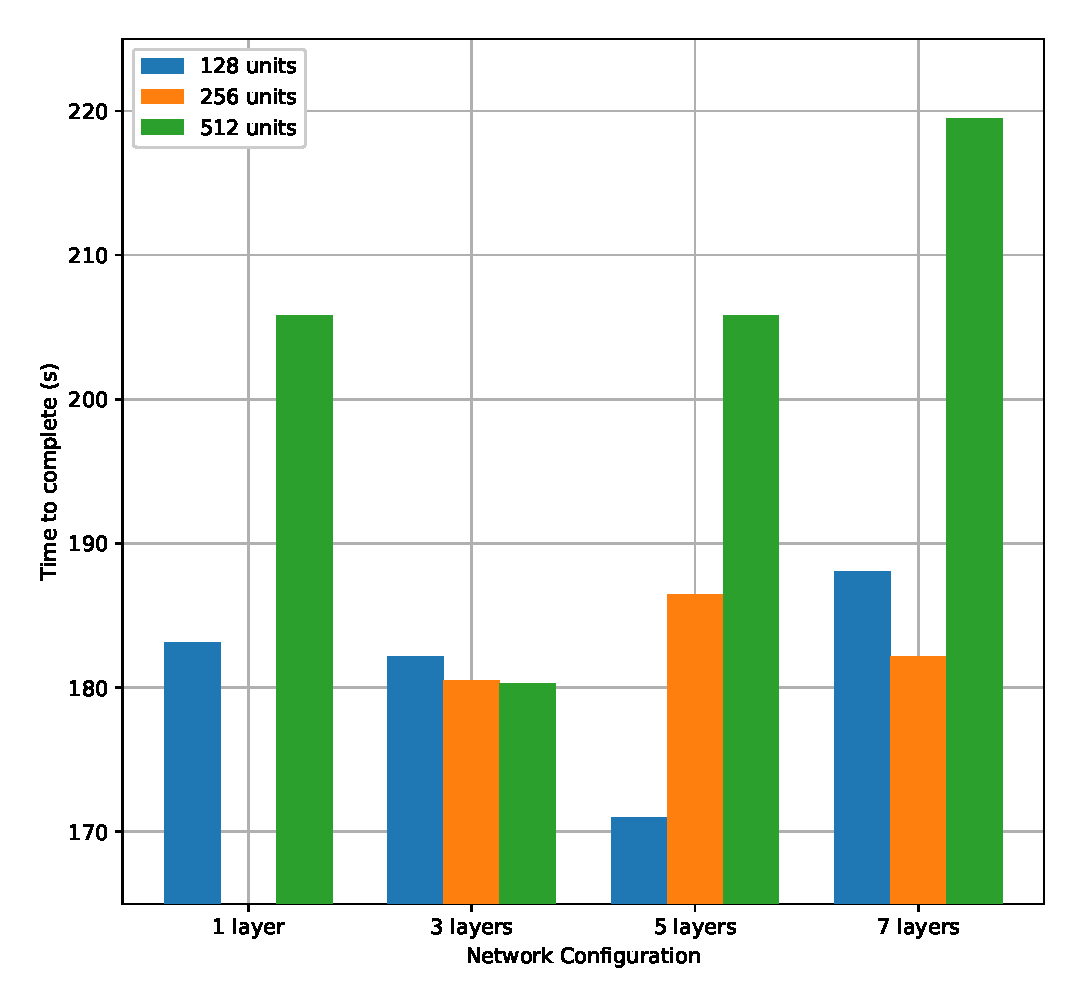
\includegraphics[width=\linewidth]{move_to_static_target_test_static_brain_bar_chart.eps}
        \caption{Test results for reaching a static target using agent that was trained to reach static targets}
        \label{test_results_static_target_static_brain_bar_chart}
    \end{center}
\end{figure}


\subsection{Agent trained to reach moving targets}

The second part of the test is measuring how well an agent that was trained to reach moving targets can also reach static targets, and if it could also beat the agent that was trained to reach static targets. The obtained results are in Table \ref{move_to_static_target_test_results:2} and Figure \ref{test_results_static_target_moving_brain_bar_chart}. Just like in the training section \ref{moving_target:training}, half of the tested agents will also have the target's direction as an observation (which is the vector $(0, 0, 0)$ since the target is not moving).

Looking at the results for the architecture with just a single hidden layer

\begin{table}
    \centering
    \begin{tabular}{|| m{11.3em} | m{10em} | m{9.6em} ||}
    \hline \hline
    \strong{Network Configuration} & \strong{Observed target's direction} & \strong{Time to complete ($s$)} \\ \hline \hline
    1 layer, 128 units & No & 192.7527 \\ \hline
    1 layer, 128 units & Yes & 196.2916 \\ \hline
    1 layer, 256 units & No & 223.6499 \\ \hline
    1 layer, 256 units & Yes & 464.985 \\ \hline
    1 layer, 512 units & No & 215.4364 \\ \hline
    1 layer, 512 units & Yes & 208.1973 \\ \hline
    3 layers, 128 units & No & 200.7101 \\ \hline
    3 layers, 128 units & Yes & 192.2111 \\ \hline
    3 layers, 256 units & No & 291.4421 \\ \hline
    3 layers, 256 units & Yes & 202.1844 \\ \hline
    3 layers, 512 units & No & 321.6053 \\ \hline
    3 layers, 512 units & Yes & 188.5515 \\ \hline
    5 layers, 128 units & No & 252.7738 \\ \hline
    5 layers, 128 units & Yes & 187.1074 \\ \hline
    5 layers, 256 units & No & 363.128 \\ \hline
    5 layers, 256 units & Yes & 215.8631 \\ \hline
    5 layers, 512 units & No & 576.1487 \\ \hline
    5 layers, 512 units & Yes & 214.0343 \\ \hline \hline
    \end{tabular}
    \caption{Test results for reaching a static target using agent that was trained to reach moving targets}
    \label{move_to_static_target_test_results:2}
\end{table}

\begin{figure}
    \begin{center}
        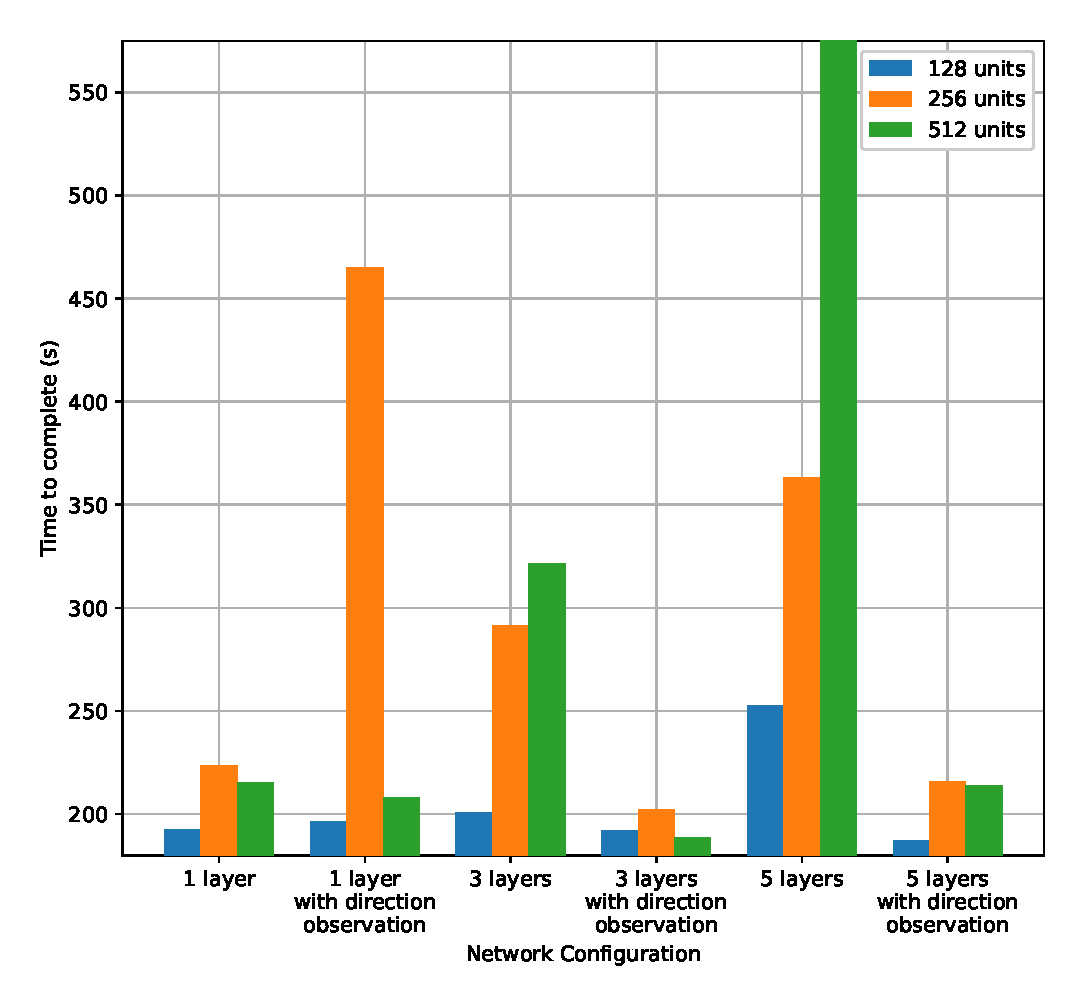
\includegraphics[width=\linewidth]{move_to_static_target_test_moving_brain_bar_chart.eps}
        \caption{Test results for reaching a static target using agent that was trained to reach moving targets}
        \label{test_results_static_target_moving_brain_bar_chart}
    \end{center}
\end{figure}






\section{Reaching a moving target}

TODO: la moving target se atinge obiectivu de 100 de ori


\subsection{Agent trained to reach moving targets}

\begin{table}
    \centering
    \begin{tabular}{|| m{11.3em} | m{10em} | m{9.6em} ||}
    \hline \hline
    \strong{Network Configuration} & \strong{Observed target's direction} & \strong{Time to complete ($s$)} \\ \hline \hline
    1 layer, 128 units & No & 482.4993 \\ \hline
    1 layer, 128 units & Yes & 499.2063 \\ \hline
    1 layer, 256 units & No & 495.7267 \\ \hline
    1 layer, 256 units & Yes & 688.592 \\ \hline
    1 layer, 512 units & No & 452.052 \\ \hline
    1 layer, 512 units & Yes & 485.6294 \\ \hline
    3 layers, 128 units & No & 484.7428 \\ \hline
    3 layers, 128 units & Yes & 488.6792 \\ \hline
    3 layers, 256 units & No & 491.0297 \\ \hline
    3 layers, 256 units & Yes & 485.8719 \\ \hline
    3 layers, 512 units & No & 602.9445 \\ \hline
    3 layers, 512 units & Yes & 467.162 \\ \hline
    5 layers, 128 units & No & 527.4669 \\ \hline
    5 layers, 128 units & Yes & 462.4213 \\ \hline
    5 layers, 256 units & No & 549.7428 \\ \hline
    5 layers, 256 units & Yes & 500.7562 \\ \hline
    5 layers, 512 units & No & 568.0677 \\ \hline
    5 layers, 512 units & Yes & 506.722 \\ \hline \hline
    \end{tabular}
    \caption{Test results for reaching a moving target using agent that was trained to reach moving targets}
    \label{move_to_moving_target_test_results:2}
\end{table}

\begin{figure}
    \begin{center}
        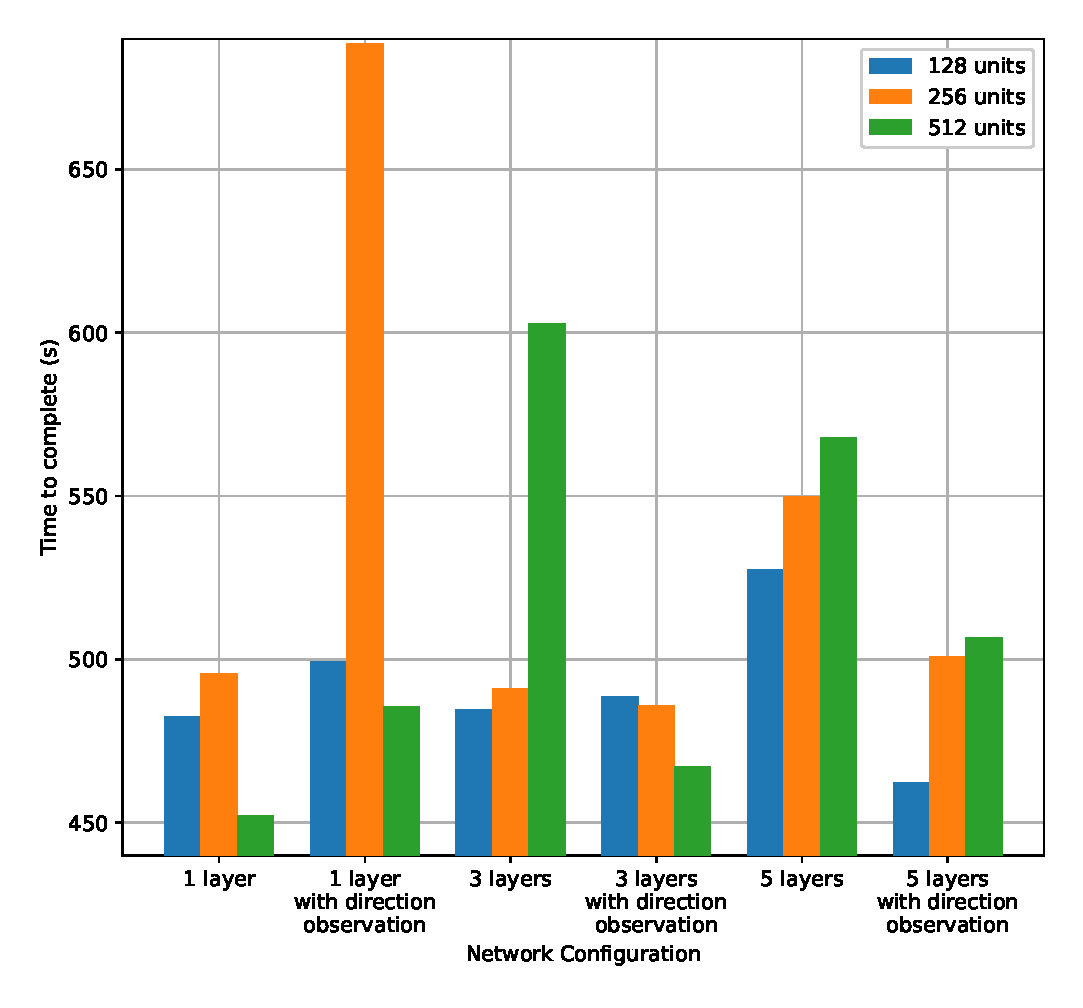
\includegraphics[width=\linewidth]{move_to_moving_target_test_moving_brain_bar_chart.eps}
        \caption{Test results for reaching a moving target using agent that was trained to reach moving targets}
        \label{test_results_moving_target_moving_brain_bar_chart}
    \end{center}
\end{figure}


\subsection{Agent trained to reach static targets}



\begin{table}
    \centering
    \begin{tabular}{|| m{15em} | m{15em} ||}
    \hline \hline
    \strong{Network Configuration} & \strong{Time to complete ($s$)} \\ \hline \hline
    1 layer, 128 units & 427.4408 \\ \hline
    1 layer, 256 units & DNF \\ \hline
    1 layer, 512 units & 438.7894 \\ \hline
    3 layers, 128 units & 450.3436 \\ \hline
    3 layers, 256 units & 457.2029 \\ \hline
    3 layers, 512 units & 448.4958 \\ \hline
    5 layers, 128 units & 429.3176 \\ \hline
    5 layers, 256 units & 466.765 \\ \hline
    5 layers, 512 units & 462.7256 \\ \hline
    7 layers, 128 units & 465.1996 \\ \hline
    7 layers, 256 units & 479.0871 \\ \hline
    7 layers, 512 units & 546.0353 \\ \hline \hline
    \end{tabular}
    \caption{Test results for reaching a moving target using agent that was trained to reach static targets}
    \label{move_to_moving_target_test_results:1}
\end{table}

\begin{figure}
    \begin{center}
        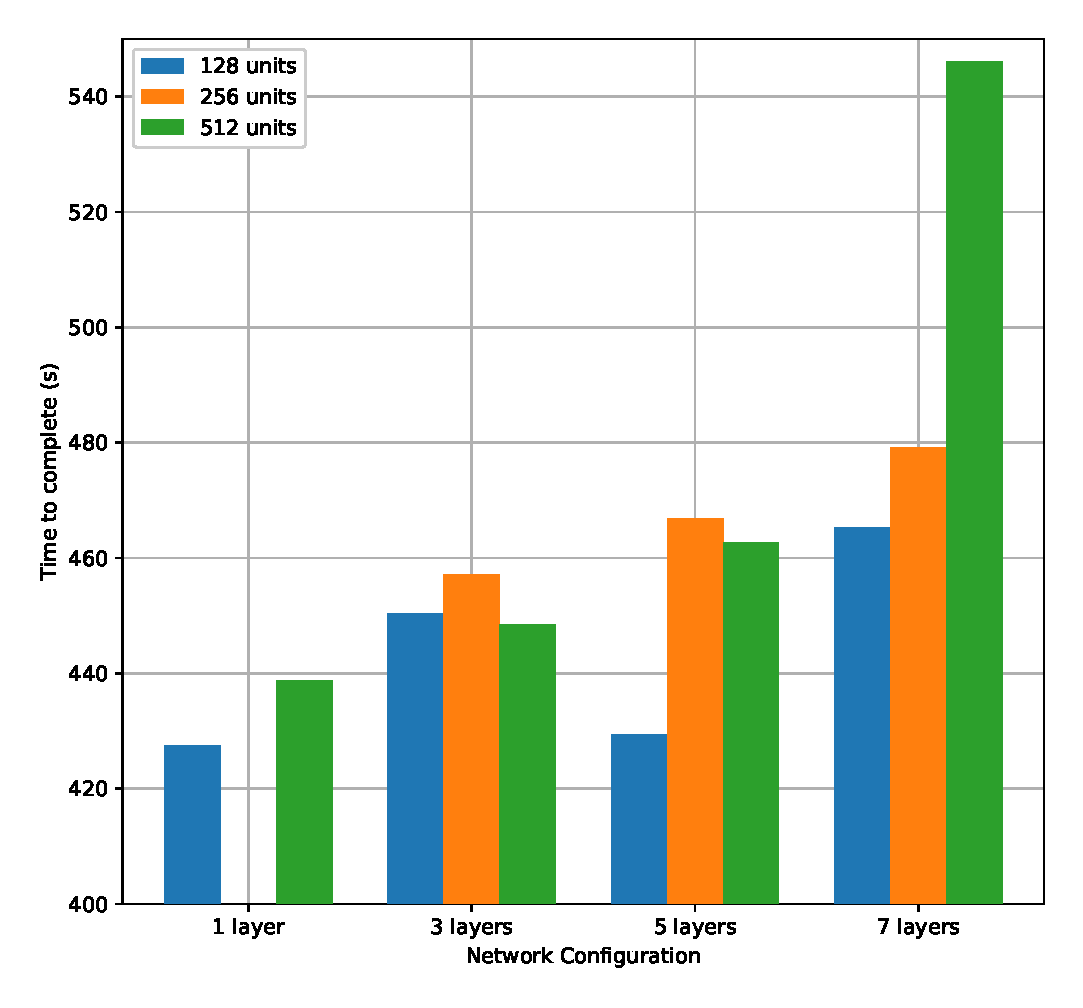
\includegraphics[width=\linewidth]{move_to_moving_target_test_static_brain_bar_chart.eps}
        \caption{Test results for reaching a moving target using agent that was trained to reach static targets}
        \label{test_results_moving_target_static_brain_bar_chart}
    \end{center}
\end{figure}



\section{Shooting a moving target}

TODO: la shooting target se impusca obiectivu de 100 de ori

\begin{table}
    \centering
    \begin{tabular}{|| m{15em} | m{15em} ||}
    \hline \hline
    \strong{Network Configuration} & \strong{Time to complete ($s$)} \\ \hline \hline
    1 layer, 128 units & 499.8927 \\ \hline
    1 layer, 256 units & 564.696 \\ \hline
    1 layer, 512 units & 536.6353 \\ \hline
    3 layers, 128 units & 590.7621 \\ \hline
    3 layers, 256 units & 637.085 \\ \hline
    3 layers, 512 units & 736.3587 \\ \hline
    5 layers, 128 units & 606.5751 \\ \hline
    5 layers, 256 units & 675.0099 \\ \hline
    5 layers, 512 units & 817.632 \\ \hline
    7 layers, 128 units & 837.6456 \\ \hline
    7 layers, 256 units & 872.1839 \\ \hline
    7 layers, 512 units & 914.4853 \\ \hline \hline
    \end{tabular}
    \caption{Test results for shooting a moving target using agent that was trained using \emph{naive} method}
    \label{shoot_moving_targets_test_results:1}
\end{table}

\begin{table}
    \centering
    \begin{tabular}{|| m{11.5em} | m{13em} | m{10em} ||}
    \hline \hline
    \strong{Network Configuration} & \strong{Bullet Observations} & \strong{Time to complete ($s$)} \\ \hline \hline
    1 layer, 128 units & Bullet's trajectory and speed & 528.1937 \\ \hline
    1 layer, 128 units & Bullet's speed & 547.2708 \\ \hline
    1 layer, 128 units & Only if bullet was fired & 499.8927 \\ \hline
    3 layers, 128 units & Bullet's trajectory and speed & 529.0487 \\ \hline
    3 layers, 128 units & Bullet's speed & 557.6132 \\ \hline
    3 layers, 128 units & Only if bullet was fired & 590.7621 \\ \hline
    5 layers, 128 units & Bullet's trajectory and speed & 628.6615 \\ \hline
    5 layers, 128 units & Bullet's speed & 688.095 \\ \hline
    5 layers, 128 units & Only if bullet was fired & 606.5751 \\ \hline
    7 layers, 128 units & Bullet's trajectory and speed & 687.3325 \\ \hline
    7 layers, 128 units & Bullet's speed & 684.9317 \\ \hline
    7 layers, 128 units & Only if bullet was fired & 837.6456 \\ \hline \hline
    \end{tabular}
    \caption{Test results for shooting a moving target using agent that was trained using \emph{naive} method and different bullet observation combinations}
    \label{shoot_moving_targets_test_results:2}
\end{table}


\begin{figure}
    \begin{center}
        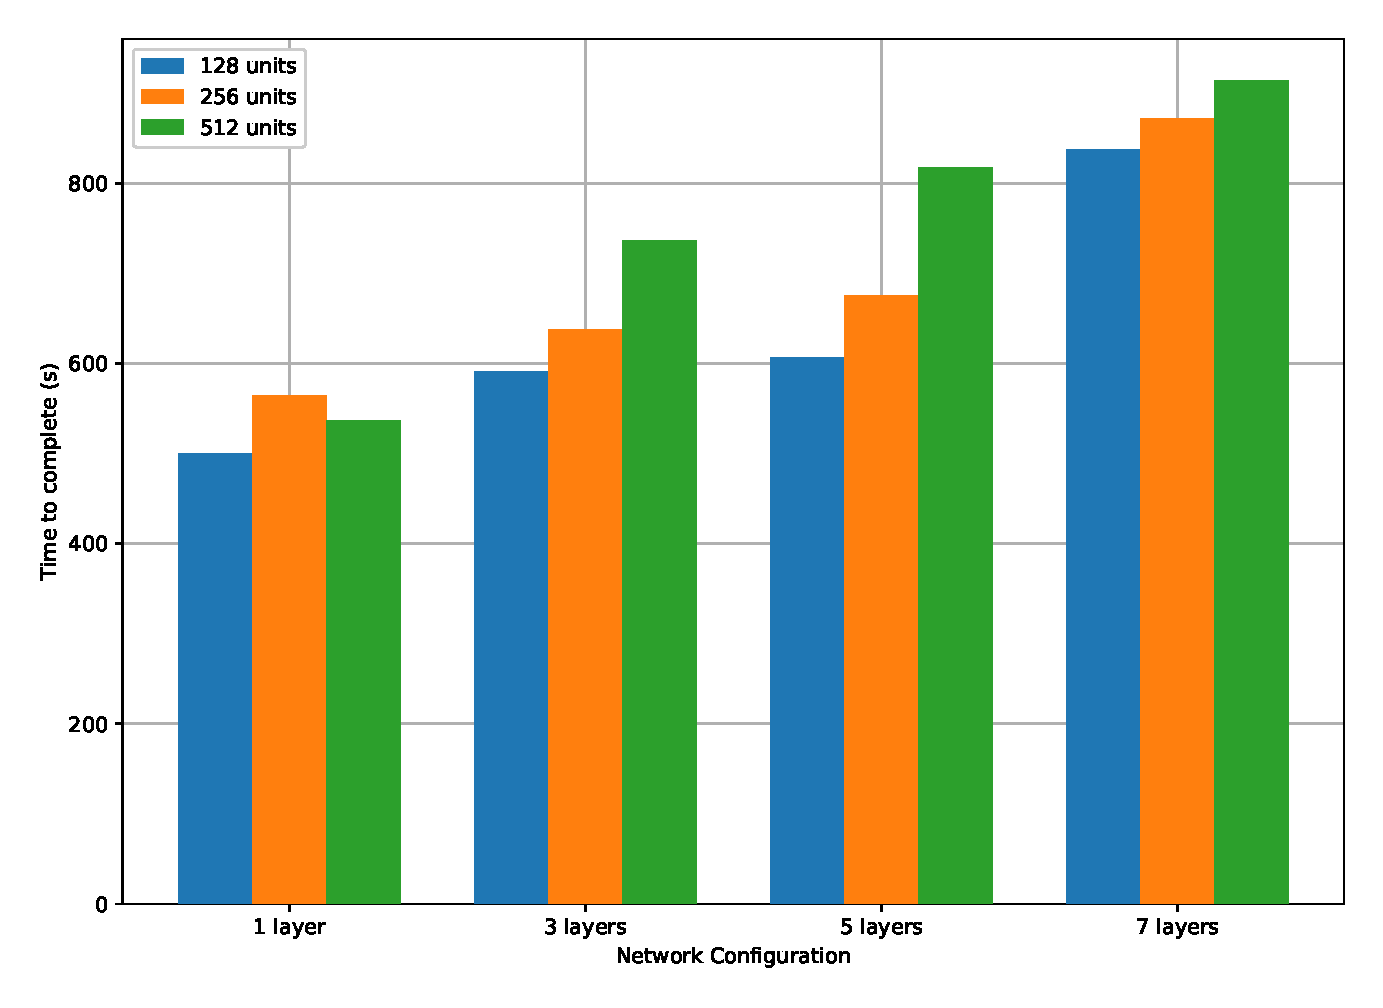
\includegraphics[width=\linewidth]{shoot_moving_target_test_bar_chart.eps}
        \caption{Test results for shooting a moving target using agent that was trained using \emph{naive} method}
        \label{test_results_shoot_moving_target_bar_chart}
    \end{center}
\end{figure}

\begin{figure}
    \begin{center}
        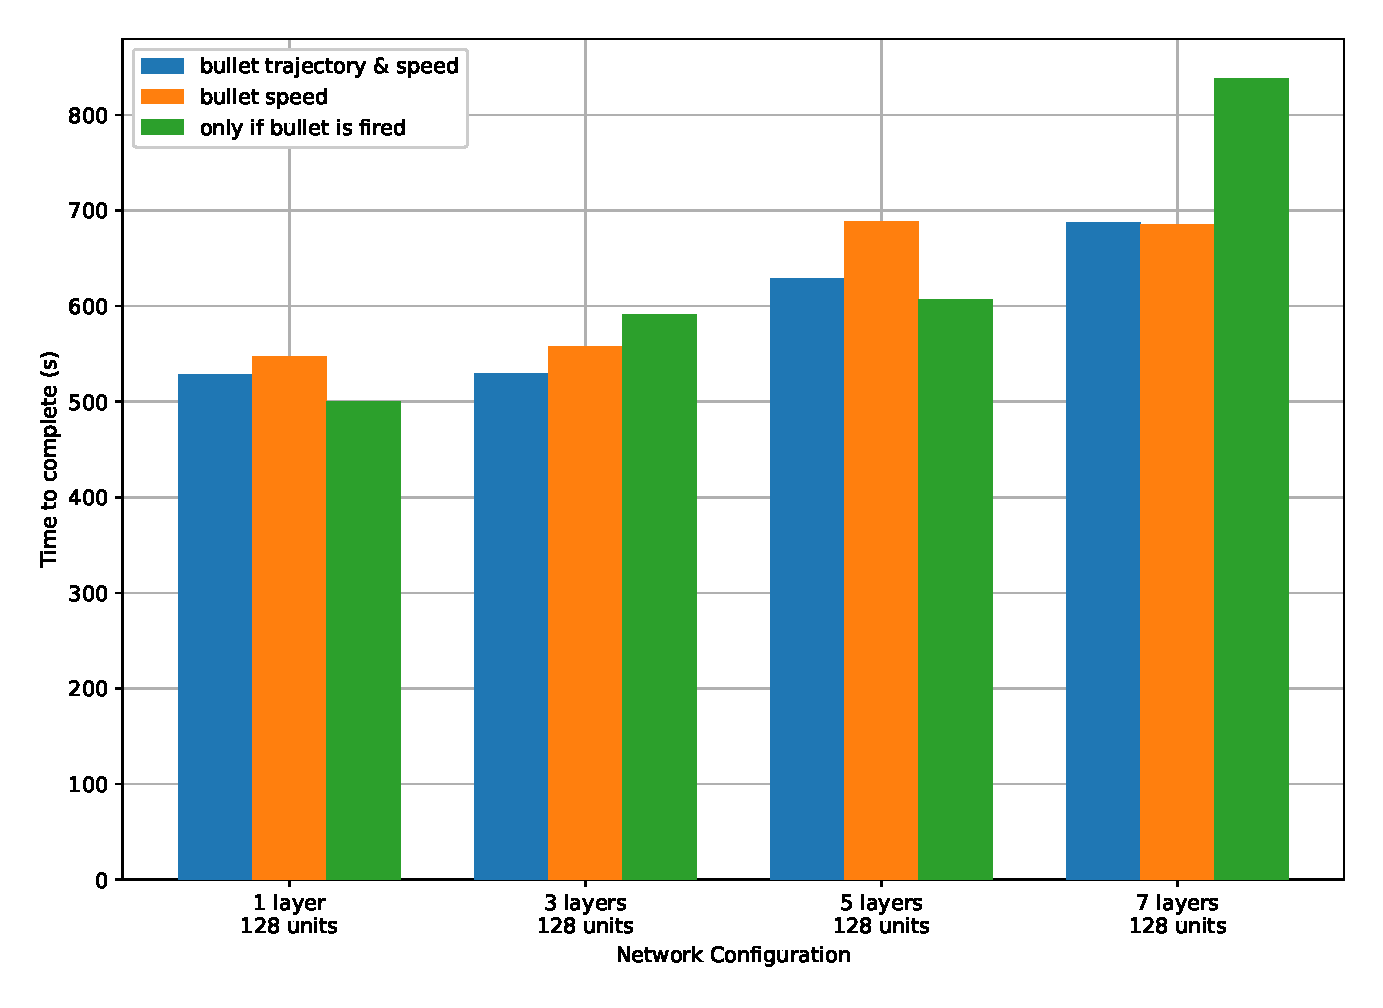
\includegraphics[width=\linewidth]{shoot_moving_target_test_obs_comparasion_bar_chart.eps}
        \caption{Test results for shooting a moving target using agent that was trained using \emph{naive} method and different bullet observation combinations}
        \label{test_results_shoot_moving_target_obs_comparasion_bar_chart}
    \end{center}
\end{figure}


\section{Fighting against an AI controlled enemy}

TODO: sa fac sa pot sa bat un tank, dupa sa vad daca paote sa bata inamicu, si daca da, sa vad cat de repede poa sa bata inamicu de x ori (eventual sa fac un mean time per round, sau sa zic de cate ori a fost lovit, etc)